\documentclass[12pt]{article}
\usepackage{latexsym}
\usepackage{fancyhdr}
\usepackage{amssymb,amsmath,amsthm}
\usepackage[pdftex]{graphicx}
\usepackage{pdfpages}
\usepackage[margin=1in]{geometry}


% Create answer counter to keep track of seperate responses
\newcounter{AnswerCounter}
\newcounter{SubAnswerCounter}
\setcounter{AnswerCounter}{1}
\setcounter{SubAnswerCounter}{1}

% Create answer environment which uses counter
\newenvironment{answer}[0]{
  \setcounter{SubAnswerCounter}{1}
  \bigskip
  \textbf{Solution \arabic{AnswerCounter}}
  \\
  \begin{small}
}{
  \end{small}
  \stepcounter{AnswerCounter}
}

\newenvironment{subanswer}[0]{
  (\alph{SubAnswerCounter})
}{
 \bigskip
  \stepcounter{SubAnswerCounter}
}

% Allows easy use of vectors
\newcommand{\vect}[1]{\vec{\boldsymbol{#1}}}

% Setting up the title
\title{Mathematics 131 \\
Topology I}
\author{
        Luis Antonio Perez \\
        HUID: 70871564 \\
        Harvard College \\
        \href{mailto:luisperez@college.harvard.edu}{luisperez@college}
}
\date{\today}

% Custom Header information on each page
\pagestyle{fancy}
\lhead{HUID: 70871564}
\rhead{Perez - \thepage}
\renewcommand{\headrulewidth}{0.1pt}
\renewcommand{\footrulewidth}{0.1pt}

% Title page is page 0
\setcounter{page}{0}

\begin{document}
%\maketitle
\pagebreak

\begin{answer}[Page 127, \#4]
\begin{subanswer}
Recall the fact that the product topology is coarser than the uniform topology which is coarser than the box topology. Then if we can show that a particular function is not continuous for a certain topology $\mathcal{T}$, then it is not continuous for any coarser topology $T' \supset T$. Firstly, note that the functions are all continuous for the product topology by Theorem 19.6. We reprove the results now:
\begin{proof}
Take $z$ to be any of our functions. Then note that $z(t) = (z_\alpha(t))_{\alpha}$ where each $z_\alpha$ is continuous on $\mathbb{R}$. Taking a typical subbasis element of $\mathbb{R}^{\omega}$ of the form $\pi_{\beta}^{-1}(U_{\beta})$ where $\beta$ is some index and $U_{\beta}$ is open in $X_{\beta}$. Then note that:
\begin{align*}
z_{\beta}^{-1}(\pi_{\beta}(U_{\beta})) = z_{\beta}^{-1}(U_{\beta})
\end{align*}
which is open by continuity of $z_\beta$.
\end{proof}
Next, we know that all three functions are not continuous in the box topology. Take the open set $U = ((-1,1), (-\frac{1}{4},\frac{1}{4}), (-\frac{1}{9}, \frac{1}{9}), \cdots, (\frac{1}{t^2}, \frac{1}{t^2}) \cdots)$ and note that $f^{-1}(U) = g^{-1}(U) = h^{-1}(U) = \{0\}$ because, no matter how small $t$ is, eventually $\frac{1}{t^2}$ is smaller than all $kt$, $t$, and $\frac{1}{kt}$ for all $k$.

Finally, we note that $g$ and $h$ are both continuous under the uniform topology while $f$ is not.
\begin{proof}
For $f$, we take the open Ball $B(0,\epsilon)$ for $\epsilon > 0$. Then note that no matter what $t$ is, the there always exists a $k$ for which $kt > \epsilon$ (in particular, we can take $k > \frac{\epsilon}{t}$. Therefore, the inverse image of this ball is $\{0\}$, which is closed, and therefore $f$ is not continuous.

For $g,h$, simply note that for any point in an open set $U$ containing points in the image of $g$, we have an open ball $B(t,\epsilon) \subset U$ such that $g^{-1}(B(t,\epsilon)) = (t - \frac{\epsilon}{2}, t + \frac{\epsilon}{2})$ which is open. Similarly, for any points in the image of $h$ contained in $U$, we have a ball $B(t,\epsilon)$ such that $h^{-1}(B(t,\epsilon)) = (t - \frac{\epsilon}{2}, t + \frac{\epsilon}{2})$ which is open. Therefore, $g,h$ are both continuous on the uniform topology.
\end{proof}
To summarize:
\begin{itemize}
\item $f$ is only continuous on the product topology.
\item $g$ is continuous on the product and uniform topology.
\item $h$ is continuous on the product and uniform topology.
\end{itemize}
\end{subanswer}
\begin{subanswer}
We discuss each element in turn. Note that if an element does not converge on a particular topology, then it doesn't converge on any finer topology. Similarly, if it converges in a topology, than it converges on all other coarser topologies.
\begin{itemize}
\item Note that $w_n$ does not converge in the uniform topology since it's distance from $0$ is always $1$ since there exists some element $>1$ in the $w_n$ for all $n$. However, it does converge in the product topology to $0 \in \mathbb{R}^{\omega}$ there exists an $N$ large enough such that $\forall w_n$ where $n > N$, the elements after the $N$-th are all contained in a ball around $0$ with $\frac{1}{k}$ as the distance.

\item Note that $x_n$ does converge in the uniform topology to $0$. This is because for any $B(0,\epsilon)$ with $\epsilon > 0$, we have that for $x_n$ where $n > \frac{1}{\epsilon}$, the first $n$ elements are all $0$ and all following elements are equal to $\frac{1}{n+1} < \frac{1}{n} < \epsilon$, so we have convergence.

However, $x_n$ does not converge in the box topology. The open set $(-\frac{1}{2},\frac{1}{2}) \times (\frac{1}{3} \frac{1}{3}) \times \cdots \times (\frac{1}{k}, \frac{1}{k}), \cdots$ contains the zero elements but does not contain any elements in the sequence since for some large enough $k$, a point in the sequence has that $k$ outside the set.

\item Note that $y_n$ does converge in the uniform topology to $0$. This is because for any $B(0, \epsilon)$ with $\epsilon > 0$, we have that for $x_n$ where $n > \frac{1}{\epsilon}$, all of the elements are a distance less than $\epsilon$ (similar argument to above). However, it again does not converge in the box topology. The same open set used to show the non-convergence of $x_n$ can be used. Note that no matter the $n$, we will have a large enough $k$ such that $\frac{1}{n} > \frac{1}{k}$.

\item $z_n$ converges in the box topology to $0 \in \mathbb{R}^{\omega}$. This is because for large enough $n$, the first two coordinates approach $0$ and all others are $0$. Therefore, every open set around the $0$ sequence contains all elements for $z_n$ for some large $n$ going forward.
\end{itemize}
\end{subanswer}
\end{answer}

\begin{answer}[Page 127, \#8]
\begin{subanswer}
We take the set around $x$ $U_x = \{y : |x_i - y_i|^2 < \frac{\epsilon^2}{2^i} \}$. Then note that $U_x$ is open in the box topology by construction, and that it is also open in the the $l^2$ topology. Since for any point $y$ in the set:
\begin{align*}
\left[\sum_{i=1}^{\infty} (x_i - y_i)^2\right] ^{\frac{1}{2}} < \left[\sum_{i=1}^{\infty} \frac{\epsilon^2}{2^i} \right]^{\frac{1}{2}} = \epsilon
\end{align*}
Furthermore, note that $U_x$ is also open in the uniform topology because the maximum distance for any point is $\frac{\epsilon^2}{2} < \epsilon$, so it is fully contained in the ball $B(x,\epsilon)$. So from the above, we have that for every $B_{\bar{\rho}}(x,\epsilon)$ in the uniform, then $B_{l^2}(x,\epsilon) \subset B_{\bar{\rho}}(x,\epsilon)$, and $U_x$ defined as above is open in the box topology and $U_x \subset B_{l^2}(x,\epsilon)$. Therefore, every open set in the uniform is open in the $l^2$ topology, and every open set in the $l^2$ topology is open in the box topology.
\end{subanswer}

\begin{subanswer}
To show that the four topologies (box, $l^2$, uniform, and product) are all different in this space, we just need to find an open set in the box topology that's not open in $l^2$ (which is therefore not open in any of the coarser topologies). Similarly, find an open set in $l^2$ which is not open in the uniform (and therefore not open in any of the coarser topologies). Lastly, we just need an open set in the uniform which is not open in the product.

First, to show the box topology $\subsetneq$ $l^2$-topology.
\begin{proof}
Take the set $U = ((-\frac{1}{2}, \frac{1}{2}), (-\frac{1}{3}, \frac{1}{3}, \cdots) \cap X$ which is open in the box topology of $X$. However, note that $\forall \epsilon > 0$, $B_{l}(0,\epsilon)$ does not contain some points in the set $U$. To see this, take the $0$ element which is contained in both $U$ and $B_{l^2}(0,\epsilon)$. Then note that $\exists k$ such that $\frac{1}{k} < \epsilon$. and therefore the point $c = (c_1,c_2,\cdots)$ given by all zeros except for $c_{k+1} = \frac{1}{k}$ is contained in $B_{l}(0,\epsilon)$ but is not contained in $U$ since $\frac{1}{k} > \frac{1}{k+1}$.

This shows that the $l^2$ topology is not finer than the box topology.
 \end{proof}
Next, we show that the $l^2$-topology $\subsetneq$ uniform topology.
\begin{proof}
Consider the open ball $B_{l^2}(0,\epsilon)$. Then note that $\forall \delta > 0$, the open ball $B_{\bar{\rho}}(0,\delta)$ contains the point $c$ with all entries $0$ except for $\frac{2\epsilon}{\delta^2} + 1$ non-zero entries each with values $c_k = \frac{\delta}{2}$. However, we have that:
\begin{align*}
\left[ \sum_{k=1}^{\infty} c_i^2 \right]^{\frac{1}{2}} > \frac{2\epsilon}{\delta^2}(\frac{\delta^2}{2}) = \epsilon
\end{align*}
Therefore this point is not contained in $B_{l^2}(0,\epsilon)$, so the set is not open in the uniform topology.
\end{proof}
Now the final part.
\begin{proof}
Suppose we have a ball $B_{\hat{\epsilon}}(0, \epsilon)$ for $0 < \epsilon < 1$. Then note that for every open set in the product topology containing this $U = U_1 \times \cdots \times U_n \times \mathbb{R} \times \mathbb{R}$ which contains the $0$ element, there exists a point $p$ which can have any values on the coordinates which project to $\mathbb{R}$, and in particular, could havel $\epsilon + 1$. Therefore, this point $p \notin B_{\hat{\epsilon}}$. This implies that the product and uniform topologies are not the same.
\end{proof}
By the above, we've shown that all of the topologies are different.
\end{subanswer}

\begin{subanswer}
We show that the box topology is finer than the $l^2$ topology on $H$.
\begin{proof}
To see this, note that the set defined by $U = ([0, \frac{1}{2}), [0,\frac{1}{4}), [0,\frac{1}{8}), \cdots)$ is open in $H$ under the box topology, since each $[0,\frac{1}{2^n})$ is open. However, for every $B(0,\epsilon)$ we can create the sequence of the form $c = (k\epsilon, \frac{k\epsilon}{2}, \frac{k\epsilon}{4} \cdots, \frac{k\epsilon}{n^2}, \cdots) \in H$ such that $c \in B(0,\epsilon)$ for constant $k$ small enough. However, $c \notin U$ because $\frac{c}{n^2} > \frac{1}{2^n}$ for large enough $n$.
\end{proof}
On the other hand, the other three topologies are equivalent. We show this by showing that the product topology is finer than the $l^2$- topology. This occurs, intuitively, because the space $H$ is bounded by a sequence convergent on smaller and smaller squares. So all the coordinates which correspond to the entire space are now bounded and shrinking.
\begin{proof}
Given a $B_{l^2}(x,\epsilon)$, create the set $U = \prod_{i = 1}^{n} (x_i - \delta, x_i + \delta) \times \prod_{i = n+1}^{\infty} [0, \frac{1}{i}]$
Then note that this set is fully contained in $B_{l^2}(x,\epsilon)$. This is because for any point $y \in U$:
\begin{align*}
d(y,x) &= \left[\sum_{i=1}^{n} \delta^2 + \sum_{i = n+1}^{\infty} \frac{1}{i^2}\right]^{\frac{1}{2}} \\
&< \epsilon \tag{for sufficiently large $n$ and sufficiently small $\delta > 0$}
\end{align*}
\end{proof}
\end{subanswer}
\end{answer}

\begin{answer}[Page 127, \#11]
Suppose $d(x,y)$ is a metric, then it is immediately clear that:
\begin{align*}
d'(x,y) = \frac{d(x,y)}{1 + d(x,y)} < 1 \tag{$\forall x,y$}
\end{align*}
so the metric is clearly bounded.

Additionally, all other properties of a metric hold trivially for $d'$ because they hold for $d$. The only difficult thing to prove is the triangle inequality.

First, we follow the hint. Note that $f$ is a strictly increasing function on $\mathbb{R}^+$ (we can take a look at the graph, or note that the derivate is given by $\frac{1}{(1+x)^2)} \geq 0$ for $x \geq 0$.
Then by the mean value theorem applied to two intervals $[0,a]$ and $[b,a+b]$ where $b > a$, we have two values $c \in [0,a]$ and $c' \in [b,a+b]$ with $c' \geq c$ where:
\begin{align*}
af'(c) &=  f(a+b) - f(b) \\
af'(c') &= f(a) - f(0) = f(a)
\end{align*}
Then we have the following:
\begin{align*}
f(a+b) - f(b) &= af'(c) \\
&\leq af'(c') \tag{$f'$ is strictly increasing} \\
&= f(a) \\
\implies f(a+b) &\leq f(a) + f(b)
\end{align*}
Now we use the fact that $d' = f \circ d$:
\begin{align*}
d'(x,z) + d'(z,y) = f(d(x,z)) + f(d(z,y)) \\
&\geq f(d(x,y)+d(y,z)) \tag{using the above} \\
&\geq f(d(x,y)) \tag{by the fact that $f$ is increasing and triangle inequality applied to $d$} \\
=d'(x,y)
\end{align*}
The above shows that $d'$ fulfills the triangle inequality.

Now we just need to show that the induced topology is equivalent to that induced by $d$. Note that $f$ is continuous on the $d$ topology, and that as composition of two continuous functions, $d'$ is therefore also continuous on the $d$ topology. Similarly, note that $f^{-1}$ is continuous on the $d'$ topology, as $d$ as a composition of two continuous functions is continuous on the $d'$ topology. This implies that the topologies are the same.
\end{answer}

\begin{answer}[Page 134, \#6]
The sequence converges point wise. If we fix $x \in [0,1)$, then we have that $\forall \epsilon > 0$, $\exists N > 0$ such that $\forall n > N$, $d(x^n,0) < \epsilon$. This implies that the sequence converges point wise.
On the other hand, we'd expect the sequence to converge uniformly to the $0$ function. However, this is not the case:
\begin{proof}
Note that for a given $\epsilon > 0$ we have a candidate $N > 0$ satisfying uniform convergence. Then simply take $x = (1- \frac{\epsilon}{N})$ and note that:
\begin{align*}
f(x) &= (1-\frac{1 - \epsilon}{N}) \\
&\geq 1 - (1 - \epsilon) \tag{using Bernoulli inequality}\\
&= \epsilon
\end{align*}
Which means our candidate $N$ is not correct. We can always choose an $x$ close enough to $1$ which makes this be the case.
\end{proof}
\end{answer}

\begin{answer}[Page 134, \#9]
\begin{subanswer}
We proof convergence point wise first. Suppose we're given a value $c \in \mathbb{R}$. Then:
\begin{align*}
\lim_{n\to \infty} \frac{1}{n^3[c - \frac{1}{n}]^2 + 1} &= \lim_{n \to \infty} \frac{1}{c^2n^3 - 2cn^2 + n - 1} \\
&= \lim_{n \to \infty} \frac{\frac{1}{n^3}}{c^2 - \frac{2c}{n} + \frac{1}{n^2} - \frac{1}{n^3}} \\
&= \frac{0}{c^2} = 0
\end{align*}
The above shows that for any fixed $c \in \mathbb{R}$, our sequence converges point wise.
\end{subanswer}

\begin{subanswer}
If the sequence converged uniformly to the zero function, then there exists an $N > 0$ such that for all $n > N$, the function is arbitrarily close to $0$ for all points $x \in \mathbb{R}$. However, simply take $x = \frac{1}{n}$ for any such $n$:
\begin{align*}
f(\frac{1}{n}) &= 1
\end{align*}
Which is clearly not arbitrarly close to $0$. Therefore, the sequence is not uniformly convergent.
\end{subanswer}
\end{answer}

\begin{answer}[Page 144, \#2]
\begin{subanswer}
We need to prove two things about the map $p: X \to Y$ in order to show that it is quotient map. The first is that $p$ is surjective.
\begin{proof}
We know that $p \circ f : Y \to Y$ is the identity map. Then note that $\forall y \in Y$, $\exists x \in X$ such that $p(x) = y$. In particular, simply note:
\begin{align*}
y &= (p \circ f)(y) \\
&= p(f(y))
\end{align*}
So $x = f(y)$.
\end{proof}
Next, we need to show that $p^{-1}(U)$ open in $X$ if and only if $U$ is open in $Y$.
\begin{proof}
Suppose $U$ is open in $Y$. Then by definition of continuity, $p^{-1}(U)$ is open in $X$.
In the other direction, suppose that $p^{-1}(U)$ is open in $X$. Then note that by continuity of $f$, we have that $f^{-1}(p^{-1}(U)) = U$ is open (this is because the inverse of the identity map is the identity).
\end{proof}
\end{subanswer}
\begin{subanswer}
Take $f: A \to X$ to be the inclusion map on $X$ for elements in $A$ since $A \subset X$. Then by the above, we have $r$ is a continuous, surjective map with a continuous map $f$ such that $r \circ f$ equals the identity on $A$. Therefore, it is a quotient map.
\end{subanswer}
\end{answer}

\begin{answer}[Page 144, \#3]
Note that the restricted map $q: A \to \mathbb{R}$ is a quotient map that is neither open nor closed. To see this, it is immediate that $q = h \circ f$ where $f: A \to \mathbb{R} \times \{0\}$ defined as $f(x,y) = (x,0)$ is a contraction and by the above problem is therefore a quotient map, and $h$ is the natural homeomorphism from $\mathbb{R} \times \{0\}$ to $\mathbb{R}$. By composition, this show that the map $q$ is a quotient map. Now we show it is neither open nor closed. If we let $U = \{(x,y) | (x,y) \in A, y > 0\}$ which is open in $A$, then $q(U) = [0,\infty]$ which is neither open nor closed in $\mathbb{R}$. Similarly, we show $q$ is not closed. Simply take the closed set $C = \{(x,\frac{1}{x}) | x \in \mathbb{R}^{+}\}$. This set is closed in $A$ with the induced topology because it's inverse is open, but $f(C) = (0,\infty)$ which is not closed.
\end{answer}

\begin{answer}[Page 144, \#4]
\begin{subanswer}
The corresponding quotient space for the equivalence class in $\mathbb{R}^2$ given by:
\begin{align*}
x_0 \times y_1 \sim x_1 \times y_1 \text{ if } x_0 + y_0^2 = x_1 + y_1^2
\end{align*}
is homeomorphic to $\mathbb{R}$. The equivalence classes defined are parabolas of the form $x + y^2= c$ where $c$ specifies the parabola uniquely. Therefore, the new topological space formed by the above equivalence class can be seen as homeomorphic to the real line. Taking any open interval $(a,b)$ specifies a set of parabolas which lie in an open set in $\mathbb{R}^2$. Similarly, taking any open set in $\mathbb{R}^2$, it just corresponds to the $c$ values for parabolas with points in the set.

More formally, and following the hint, note that $g(x \times y) = (x + y^2, 0)$ is a retraction which is a quotient map (see above). Then note that a natural homeomorphism exists from $\mathbb{R} \times \{0\}$ to $\mathbb{R}$.
\end{subanswer}

\begin{subanswer}
The corresponding quotient space for the equivalence class in $\mathbb{R}^2$ gives by:
\begin{align*}
x_0 \times y_1 \sim x_1 \times y_1 \text{ if } x_0^2 + y_0^2 = x_1^2 + y_1^2
\end{align*}
is homeomorphic to $\mathbb{R}^+ \cup \{0\}$. To see this, note that the equivalence classes are simple given by circles, each of radius $r$. Therefore, we have a direct mapping from the circles on the plane to all non-negative values by calculating the radius of the equivalence class you belong to.

More formally, note that $g(x \times y) = (x^2 + y^2, 0)$ is a retraction which is a quotient map (see above). This is naturally homeomorphic to $\mathbb{R}^+ \cup \{0\}$.
\end{subanswer}
\end{answer}


\begin{answer}[Page 145, \#1]
We proof the forward direction.
\begin{proof}
Suppose $H$ is a topological group. Then we consider the map $\times' : H \times H \to H$ given by $x \cdot y^{-1}$. Note that this is map is the composition of $\times: H \times H \to H$ given by $x\cdot y$ and $^{-1}: H \to H$ given by $x^{-1}$ where we compose the second coordinate input into $\times$. So essentially, we have $\times'(x,y) = \times(x,^{-1}(y))$. This is the composition of two continuous functions, and is therefore also continuous.
\end{proof}
Now we proof the backward direction:
\begin{proof}
Suppose that the operation $\times'$ is continuous. Then it is continuous in both variables. This implies that $^{-1}(y) = \pi_2(\times'(1,y))$, which is the composition of continuous functions, so $^{-1}$ must be continuous.
Similarly, we have $\times(x,y) = \times'(x, ^{-1}(y))$ which is again the composition of two continuous functions so is itself continuous.
\end{proof}
This completes both directions of the argument.
\end{answer}

\begin{answer}[Page 145, \# 2]
We tackle each in turn.
\begin{itemize}
\item $(\mathbb{Z}, +)$. We've previously shown that $\mathbb{Z}$ is Hausdorff (trivial to see it satisfies $T_1$, even if we didn't know it was Hausdorff because each point is an open set in $\mathbb{Z}$ as is by definition separated). Similarly, the $+: \mathbb{Z} \times \mathbb{Z} \to \mathbb{Z}$ is continuous.
\begin{proof}
Taken any sequence $(x_n,y_n)$ of integers which converges to an integer. Then note that $x_n + y_n$ is an integer, and this new sequence also converges to an integer.
\end{proof}
Additionally, $f(x) = -x$ is also continuous, where this is simply negation of the identity map.
\item $(\mathbb{R}, +)$. We've also shown that $\mathbb{R}$ is Hausdorff, but it is easy to see that it satisfies the $T_1$ separation axiom by its denseness. Again, negation is trivially continuous, and for the sum, consider:
\begin{proof}
The normal sum function is continuous. Take any sequence $(x_n,y_n)$ which converges to $(x,y)$. Then there exists an $N > 0$ such that for all $n \geq N$, each of the coordinates is within $\frac{\epsilon}{2}$ of its limit point. Then applying the sum operation, $x_n + y_n$ lies within $\epsilon$ of $x + y$. Therefore, the sum operation is continuous.
\end{proof}
\item $(\mathbb{R}^+, \cdot$). As a subspace of $\mathbb{R}$, this is also Hausdorff. In this situations, the product of two positive numbers is also positive, and the product function is continuous.
\begin{proof}
Consider a sequence $(x_n,y_n)$ which converges to $(x,y)$ and suppose $0 < \epsilon < 1$. Then there exists $N > 0$ such that $\forall n \geq N$, we have that each coordinate is within $\frac{\epsilon}{3(|x| + |y| + 1)}$ of it's limit point. Then following the hint, we have that:
\begin{align*}
d(xy, x_ny_n) &\leq |x||y_n - y| + |y||x_n - x| + |x_n - x||y_n - y|\\
&< |x|\frac{\epsilon}{3(|x| + |y| + 1)} + |y|\frac{\epsilon}{3(|x| + |y| + 1)} + \frac{\epsilon}{3(|x| + |y| + 1)}\frac{\epsilon}{3(|x| + |y| + 1)} \\
&= \frac{\epsilon}{3} \left(\frac{3(|x| + |y| + 1)(|x| + |y| + 1)}{3(|x| + |y| + 1)(|x| + |y| + 1)} \right) \\
&= \frac{\epsilon}{3} < \epsilon
\end{align*}
\end{proof}
Similarly, the inverse of the produce (ie, $\frac{1}{x}$) is continuous for $x > 0$.
\begin{proof}
Consider the open interval $(a,b) \in \mathbb{R}^+$. Then the inverse image is simply given by $(\frac{1}{b}, \frac{1}{a})$ which is also open in $\mathbb{R}^+$, thereby showing continuity.
\end{proof}
\item There's a natural homeomorphism from $S^1$ to the unit circle in $\mathbb{R}^2$, and this space is Hausdorff (and satisfies $T_1$), so $S^{1}$ satisfies $T_1$. For the continuity of the product, note that:
\begin{proof}
We can represent each complex number as $x = e^{i\theta}$ and $y = e^{i\phi}$ which $1-1$ if we restrict $\theta,\phi \in [0,2\pi)$. Then the product operation $\dot(x,y) = e^{i\theta}e^{i\phi} = e^{i(\theta + \phi\mod 2\pi)}$ which is the composition of two continuous function and is therefore continuous (recall that the sum is continuous and $e^x$ is continuous.
\end{proof}
The inverse is also continuous. This is because given a number $z = e^{i\theta}$, the inverse is simply $e^{-i\theta}$ (again, restricting $\theta \in [0,2\pi)$, which is continuous.
\item Since we're considering simply a subset of $\mathbb{R}^2$ with the normal topology, then this is immediately Hausdorff (and satisfies $T_1$ axiom). The product of two matrices is simply the composition of the normal product and sum operations in $\mathbb{R}$, so we have that it is continuous for each entry, and therefore continuous for the matrices. Similarly for the inverse, this is a composition of sum, product, and inverse in $\mathbb{R}$ ($\mathbb{R} - \{0\}$ for the inverse), so it is also continuous and by non-singularity of the matrix $A$, $A^{-1}$ exists.
\end{itemize}
\end{answer}

\begin{answer}[Problem 1]
\begin{subanswer}
The equivalences classes are given by circles centered at the origin with different radii. The below is an image shamelessly stolen from the internet.
\begin{center}
  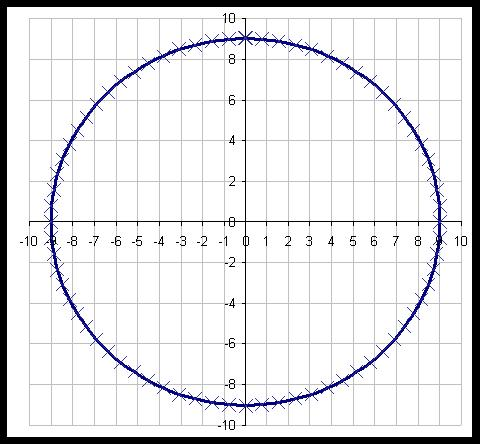
\includegraphics[scale=0.4]{circle}
\end{center}
\end{subanswer}

\begin{subanswer}
Consider and open interval of $\mathbb{R}^+ \cup \{0\}$. Suppose the open interval $(a,b)$ does not contain $0$. Then the inverse image in $G$ is the set of equivalence classes $\{\bar{(x,y)} | x^2 + y^2 = c^2, c \in \text{ interval} \}$. Note that this set is open in $\mathcal{G}$ because the set of points that map to these equivalence classes in $\mathbb{R}^2$ is open. It consists of $\{(x,y) | a < x^2 + y^2 < b\}$.

Now, suppose the open interval does contain $0$. Then it is of the form $[0,b)$. The set of equivalences classes is defined the same as above, but now the set is open because the points in $\mathbb{R}^2$ is $\{(x,y) | x^2 + y^2 < b\}$ which defines an open circle in $\mathbb{R}^2$ and is therefore open.
\end{subanswer}

\begin{subanswer}
From the above, we already know that $r$ is continuous. We just need to show that $r^{-1}$ is continuous, and we will have shown a homeomorphism. First, note that $r$ is $1-1$ since for all points $x \sim y$ in $\mathbb{R}^2$, by definition of the equivalence, the sum of their squares must be equal, and therefore the square roots of the sums are equal, and the square root function is invertible on $\mathbb{R}^+ \cup \{0\}$.

Take any open set of equivalence classes in $\mathcal{G}$ under the quotient topology. This means that we take sets of open ``donuts'' in $\mathbb{R}^2$ where a donut need not have a whole in the middle. Note that each such donut will map to an open interval $(a,b)$ where $b$ is the least upper bound of the radii and $a$ the greatest lower bound of the radii. If the donut does not have a whole in the center, then it maps to $[0,b)$ which is also open in our space by the induced topology.

The above shows that both $r$ and $r^{-1}$ are continuous (they both preserve open sets under the inverse image) and therefore $r$ is a homeomorphism.

\end{subanswer}
\end{answer}
\begin{answer}[Problem 2]
\begin{subanswer}
Suppose $a \in [0,1]$ but $a \notin C$. Then $\exists$ an $N > 0$ such that $a \notin C_n$ for all $n \geq N$ because $C_{n+1} \subset C_n$. Therefore, $a$ must belong to some open interval which we removed because it was part of the middle third. This is the case for all $a \notin C$, therefore $C^c$ is open, which implies $C$ is closed.
\end{subanswer}

\begin{subanswer}
We can take the sequence $\{c_i\}$ to be the same sequence constructed by noting that if $c \in \mathcal{C}$, then we can write $c$ as the ternary expansion with coefficients $(a_1,a_2,\cdots)$. Then each $c_i$ can just be the value for which the ternary expansion $(b_1,b_2, \cdots)$ matches the first $i$ coefficients of $c$, and consists of $0$s afterwards. This sequence converges to $c$ in the standard metric.
This is because of the following fact:
\begin{align*}
|c - c_i| &\leq \sum_{k=i+1}^{\infty} \frac{2}{3^k} \\
&= \frac{2}{3^{i+1}}\sum_{k=0}^{\infty} \frac{1}{3^k} \\
&= \frac{1}{3^i}
\end{align*}
So $|c - c_i|$ approaches $0$ for sufficiently large $i$. Additionally, by construction, each $c_i \in \mathcal{C}$ and no $c_i = c$.
\end{subanswer}

\begin{subanswer}
We use the properties of the Cantor set. As discussed in the problem statement, any point $x \in \mathcal{C}$ can be written as the ternary expansion $(a_1,a_2, \cdots)$ such that all $a_k \in \{0,2\}$. Therefore, to construct a sequence $\{x_i\} \subset [0,1] - \mathcal{C}$ that converges to $x$, we can create points $x_i = (b_1, b_2, \cdots)$ such that for the first $i - 1$ elements, we have $b_k= a_k$ for all $k < i$, with $b_{i} = 1$, and all remaining $b_k = 0$ for $k > i$. By construction, note that for any neighborhood around $x$, we can find a $i$ large enough such that all subsequent $x_i$ are fully contained within it (using the standard topology on $\mathbb{R}$).

This is because of the following fact:
\begin{align*}
|x - x_i| &\leq \frac{1}{3^i} + \sum_{k=i+1}^{\infty} \frac{2}{3^k} \\
&= \frac{1}{3^i} + \frac{1}{3^i} \\
&= \frac{2}{3^i}
\end{align*}
Therefore the sequence of $x_i$ converge to $x$.

However, by construction, each $x_i$ is not in the Cantor set because it contains a single $1$ at the $i$-th position.
\end{subanswer}

\begin{subanswer}
We follow the process outlined in the problem statement. The first step is to prove that the described map $f: [0,1] \to \mathcal{C}$ is injective. This means that $\forall x,y \in [0,1]$, if $f(x) = f(y)$, then $x = y$. To see this, note that if $c \in \mathcal{C}$ is in the image of $f$, then it cannot be written in tertiary notation with an infinite tail of $2$s. Therefore, it must be the case that $c \in f([0,1])$ must terminate in an infinite tail of $0$s. Given this, then $f(x) = f(y)$ must necessarily must each have some index at which the $0$s start. Therefore, if these two values are equal, all the locations of the $2$s must match in the tertiary expansion (recall that we cannot have infinite tails of $2$s in the image of $f$, and this avoids the problem where $0.1_3 = 0.02\cdots_3$). Therefore, each $2$ element must match in position. Taking each of those $2$ elements and converting them to $1$s, we have $x,y$ respectively (if we now consider the value in base $2$). Since all $2$s occurred in the same location, all $1$s must occur in the same location. Therefore $x = y$.

Given the above, we have shown that $f$ is injective. Therefore, because the domain $[0,1]$ is uncountable, it must be the case that the cardinality of $f([0,1]) \subset \mathcal{C}$ is the same. Therefore, the cardinality of $\mathcal{C}$ which is a subset of $[0,1]$ must, as it is sandwiched between the two, be the same cardinality as $[0,1]$. The unit interval is uncountable, therefore we have that $\mathcal{C}$ is uncountable.
\end{subanswer}
\end{answer}
\end{document}